\documentclass{article}
\usepackage{iclr2026_conference,times}

\usepackage{amsmath,amssymb,amsfonts,amsthm,mathtools}
\usepackage[utf8]{inputenc}
\usepackage[T1]{fontenc}
\usepackage{hyperref}
\usepackage{url}
\usepackage{booktabs}
\usepackage{microtype}
\usepackage{xcolor}
\usepackage{graphicx}
\usepackage{enumitem}
\usepackage[capitalize,noabbrev]{cleveref}
\crefname{proposition}{Proposition}{Propositions}
\crefname{definition}{Definition}{Definitions}

\theoremstyle{plain}
\newtheorem{theorem}{Theorem}[section]
\newtheorem{proposition}[theorem]{Proposition}
\theoremstyle{definition}
\newtheorem{definition}[theorem]{Definition}
\theoremstyle{remark}
\newtheorem{remark}[theorem]{Remark}

% Anonymous submission (default). Uncomment for camera-ready:
% \iclrfinalcopy

\title{The Compiled-Wiki Lifecycle: Certified Compilation,\\ Maintenance, and Retraction for Evolving Corpora}

\author{NatBrian}

\begin{document}
\maketitle

\begin{abstract}
Compiling a corpus into an LLM-written, self-maintaining wiki --- rather than retrieving from raw chunks at query time --- has been proposed as a replacement for RAG on evolving corpora \citep{karpathy2026wiki}. We study what such a compiled store needs beyond a good initial compile: a way to know it is still current, a way to update it without silently destroying what it already knows, and a way to remove something from it that must go. We present empirical evidence for a four-stage lifecycle --- \emph{compile, certify, maintain, retract} --- validated across real third-party systems (LightRAG, RAPTOR, a faithfully-reproduced third-party LLM-Wiki update policy) and two datasets (HoH, SciFact-Open). Compiling with recency-aware supersession resolution nearly eliminates staleness error (SER $0.007$ vs.\ $0.277$--$0.280$ for vector-RAG and graph-RAG baselines, $n{=}300$); a controlled dissociation shows the operative variable is resolution, not memory or graph structure. A finite-sample $(\delta,\varepsilon)$ contract, corrected for noisy LLM judges, certifies fidelity and currency under incremental maintenance at $40$--$47\%$ of full-audit cost, and exposes two failure modes worth naming: a \emph{build lottery} where nominally identical compiles disagree on $17$--$23\%$ of claims, and an \emph{adaptivity trap} where self-audited repair overclaims true retention by $52$ points. A minimal offline-trained maintainer beats the best prompted maintainer at equal deploy cost ($+0.127$ retention, $p{=}0.009$) without being reward-gameable at slack budgets, and a per-batch anytime-valid retention bound (LossGate) wraps any maintainer with a certified floor that rejects harmful updates, lifting retention by $0.12$--$0.14$ over the same maintainer ungated. Finally, we show that retracting a fact from an agent's memory does not make it stay retracted: a correctness-gated deletion leaves $99.0\%$ of retracted facts recoverable through the agent's own memory-consolidation loop --- statistically indistinguishable from no deletion at all --- while a cheap, weight-free membership-keyed veto reduces recoverability to $0.0\%$, matching a never-ingested oracle. We report every result with the seed count, statistical test, and scope it actually has, and we are explicit about what is not yet established: single-build variance in the compile stage, an untested half of a maintenance boundary law, and an open problem in formally certifying retraction of claims fused across multiple sources. Code, data pointers, and a reproduction guide for every stage accompany this paper.

\end{abstract}

\section{Introduction}
\label{sec:intro}

Retrieval-augmented generation answers a query by re-reading raw source chunks at serving time. This is simple and, because it never modifies what it read, hard to corrupt: every answer is grounded in whatever the retriever pulled back at that moment. It is also wasteful and structurally blind to change --- if a fact has been superseded, RAG has no mechanism to prefer the new version over the old one unless the retriever happens to rank recency, and most do not.

An alternative pattern, popularized by Karpathy as an ``LLM-Wiki'' \citep{karpathy2026wiki}, compiles a corpus once (and re-compiles or incrementally updates it as new documents arrive) into a curated, LLM-written store: a wiki that an LLM reads and rewrites, rather than a chunk index an LLM merely searches. Compiling gives a system the chance to resolve contradictions once, at write time, instead of re-litigating them on every query. That chance is also the risk: a compiled store that gets this wrong does not just retrieve a stale chunk, it \emph{writes a stale answer into the store itself}, and every subsequent query inherits the error.

This paper asks what a compiled store needs in order for that promise to be trustworthy rather than merely convenient. We organize the answer as a four-stage lifecycle, each stage validated by an independent line of experiments:

\begin{itemize}[leftmargin=1.4em,itemsep=0.2em]
\item \textbf{Compile} (\S\ref{sec:compile}): does compiling actually fix the failure mode RAG has --- answering with a superseded fact --- and is the fix coming from having a wiki (structure, memory) or from something narrower?
\item \textbf{Certify} (\S\ref{sec:certify}): once compiled, how does a store's owner or consumer know, with a stated confidence level rather than a point estimate, how much of it is still right?
\item \textbf{Maintain} (\S\ref{sec:maintain}): as new documents force the store to be rewritten, how much of what it already knew survives the rewrite, and can maintenance be made both cheap and hard to game?
\item \textbf{Retract} (\S\ref{sec:retract}): when a source is withdrawn or a fact must be removed for a real reason (legal, safety, correction), does removing it from the store actually make it stay gone?
\end{itemize}

Each stage is validated with its own benchmark and real systems, and in one case cross-checked against an independent third-party tool for external validity. This paper has not been externally peer-reviewed; every result was subjected to internal scrutiny and is reported only to the extent it survives that scrutiny. Rather than present the strongest-sounding number for each stage, we state exactly what statistical support each claim has, and are explicit in \S\ref{sec:limitations} about what is asserted but not yet run. We believe this is the more useful contribution: a lifecycle view of what actually needs to be true for a compiled knowledge store to be safe to depend on, grounded in real numbers with their real caveats attached, rather than a single headline result.

\textbf{Contributions.} (1) A controlled dissociation showing that recency-aware \emph{resolution}, not graph structure or persistent memory, is what eliminates staleness in compiled stores, validated against two real structured RAG systems (\S\ref{sec:compile}). (2) A finite-sample, noisy-judge-corrected statistical contract for compiled-store fidelity and currency, maintainable incrementally at a fraction of full-audit cost, which surfaces and quantifies two failure modes --- build-to-build disagreement and self-audit overclaiming --- that a point-estimate evaluation would miss entirely (\S\ref{sec:certify}). (3) Evidence that faithful maintenance under repeated rewriting is partially trainable at equal deploy cost, wrapped in a per-batch anytime-valid retention bound that catches and rolls back harmful updates rather than only measuring damage after the fact (\S\ref{sec:maintain}). (4) A demonstration that retraction from an agent's compiled memory is not durable under the agent's own consolidation loop unless the deletion gate is keyed on membership rather than correctness, with a fix that reduces recoverability from statistically-indistinguishable-from-no-deletion to matching a never-ingested oracle (\S\ref{sec:retract}).

\section{Compile: supersession, not memory or structure}
\label{sec:compile}

\subsection{Setup}

We use HoH \citep{ouyang2025hoh}, a benchmark built from Wikipedia dynamic-fact edits mined via token-level diffs, so that every item ships both a current and a superseded passage. We pool all evidence from $n{=}300$ HoH queries into a single shared $628$-document corpus ingested in one fixed order, rather than giving each query its own mini-corpus, so that every system under test sees the same evolving-corpus ingestion problem. Seven arms are compared under a fixed Qwen2.5-14B reader: closed-book (no retrieval), full-context dump, vector RAG (dense retrieval, top-$k$), LightRAG \citep{guo2025lightrag} (a real graph-RAG system, unmodified), RAPTOR \citep{sarthi2024raptor} (a real tree-RAG system, unmodified), an LLM-Wiki compile (Karpathy-style: an LLM reads new documents and rewrites affected pages, resolving contradictions with newer-supersedes-older), and a label-free recency resolver (a lighter-weight baseline that reorders retrieved evidence by inferred recency without a full compile step). The metric is staleness error rate (SER): the fraction of queries answered using the superseded fact instead of the current one.

\subsection{Compiling with resolution beats retrieval, structure alone does not}

\begin{table}[t]
\centering
\small
\caption{Staleness error rate (SER, lower is better) by arm, HoH $n{=}300$, Qwen2.5-14B. LLM-Wiki resolves supersession at compile time; LightRAG and RAPTOR are real structured (graph/tree) RAG systems that accumulate rather than resolve.}
\label{tab:compile-arms}
\begin{tabular}{lccc}
\toprule
Arm & Mechanism & SER & Accuracy \\
\midrule
Closed-book & no retrieval & 0.043 & 0.06 \\
Full-context dump & no selection & 0.143 & -- \\
Vector RAG & flat, accumulate & 0.277 & -- \\
LightRAG \citep{guo2025lightrag} & graph, accumulate & 0.280 & -- \\
RAPTOR \citep{sarthi2024raptor} & tree, accumulate & 0.177 & -- \\
Label-free resolver & flat, resolve & 0.050 & 0.673 \\
LLM-Wiki (ours) & flat, resolve (compiled) & \textbf{0.007} & 0.910 \\
\bottomrule
\end{tabular}
\end{table}

Closed-book abstains rather than answering correctly (accuracy $0.06$), so its low SER reflects not-answering, not currency --- it is not a real competitor. Among arms that actually answer, LLM-Wiki's SER of $0.007$ is $25$--$40\times$ lower than vector RAG ($0.277$) and the two real structured systems, LightRAG ($0.280$) and RAPTOR ($0.177$).

The obvious confound is that LLM-Wiki has both more structure (a compiled, curated store) and a different update rule (resolve instead of accumulate) than vector RAG, so the improvement could be credited to either. We break this apart with a controlled $2\times2$ over structure (flat vs.\ graph) and update policy (accumulate vs.\ resolve): flat-accumulate SER $0.277$, flat-resolve $0.050$, graph-accumulate $0.137$, graph-resolve $0.003$. Holding structure fixed and switching only the update policy from accumulate to resolve cuts SER by $5$--$45\times$ in both the flat and graph conditions; holding the update policy fixed and adding graph structure does not reliably help (flat-resolve $0.050$ vs.\ graph-resolve $0.003$ is a further improvement, but flat-accumulate $0.277$ vs.\ graph-accumulate $0.137$ shows structure alone, without resolution, still leaves the majority of staleness error in place). The operative variable is \emph{recency-aware supersession resolution}, not memory, not graph structure, and not the presence of a compile step per se — a label-free resolver with no compile at all already gets most of the way there (SER $0.050$).

\paragraph{A currency certificate, not just a point estimate.} A single SER number invites overclaiming from a lucky sample. We additionally report a Clopper-Pearson $95\%$ one-sided upper confidence bound $\hat\varepsilon$ on SER for each arm (\Cref{fig:compile-cert}): resolving arms certify $\hat\varepsilon \le 0.08$ (LLM-Wiki $0.021$; label-free resolver $0.076$--$0.080$ after judge-noise correction), while every cumulative-index (accumulating) arm certifies only $\hat\varepsilon \ge 0.18$ even though its point estimate can look better on a given sample. This certificate --- and what it costs to tighten as a function of audit size $n$ --- becomes the building block for \S\ref{sec:certify}.

\begin{figure}[t]
\centering
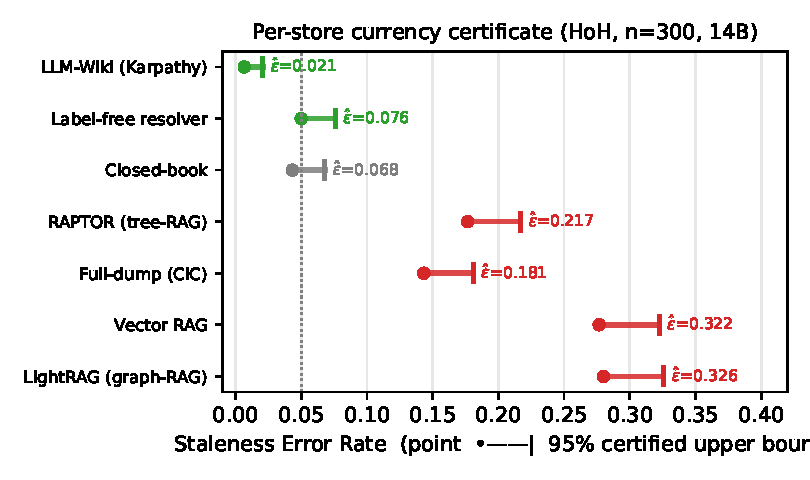
\includegraphics[width=0.48\linewidth]{figures/compile_certificate.pdf}
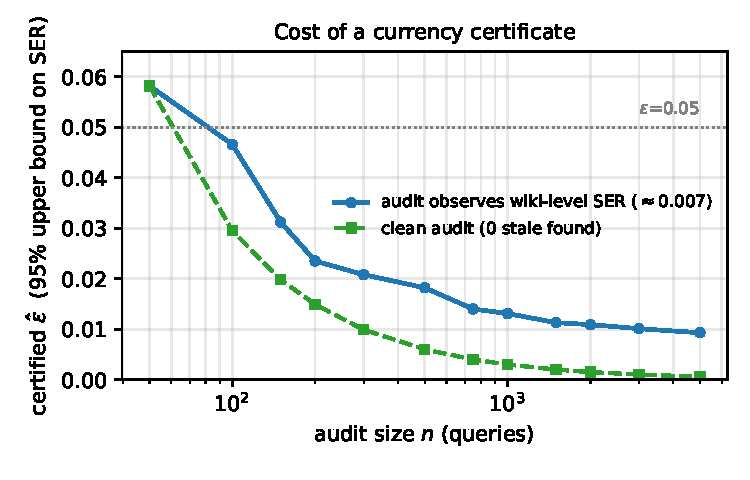
\includegraphics[width=0.48\linewidth]{figures/compile_samplesize.pdf}
\caption{Left: per-store currency certificate (point SER vs.\ $95\%$ Clopper-Pearson upper bound), resolving arms (green) vs.\ accumulating arms (red). Right: cost of tightening a currency certificate as audit size $n$ grows.}
\label{fig:compile-cert}
\end{figure}

\subsection{External validation: a different dataset, a different tool}
\label{sec:compile-external}

The result above uses one dataset (HoH), one reader model family, and our own compile harness. As an independent robustness check, we ran a second experiment on a different dataset (SciFact-Open \citep{scifact}, real PubMed abstracts, $75$ tracked SUPPORT claims plus $1500$ filler documents) using a driver that faithfully reproduces a real, independently-published third-party LLM-Wiki tool's update policy (a Hermes-style LLM-Wiki skill's documented rewrite instructions), rather than our own compile prompt. This tests whether ``iterated rewriting loses information'' is an artifact of our specific harness or a more general property of the compile-and-rewrite pattern.

\begin{table}[h]
\centering
\small
\caption{External validation on SciFact-Open, seed $=0$, single run per arm. $r_0{\to}r_T$ is retention at round $0$ vs.\ round $12$; rebuild is a fresh recompile at round $T$ with no rewrite history (the ceiling). Because arms were run independently, $r_0$ is not matched across arms --- relative retention $r_T/r_0$ is the fair cross-arm comparison.}
\label{tab:compile-external}
\begin{tabular}{lcccc}
\toprule
Arm & $r_0$ & $r_T$ & rebuild ceiling & $r_T/r_0$ \\
\midrule
Plain (large model) & 17.3\% & 13.3\% & 26.7\% & 77\% \\
Harness (rollback-wrapped, large) & 32.0\% & 29.3\% & 53.3\% & 92\% \\
Plain (small model) & 22.7\% & 2.7\% & 49.3\% & 12\% \\
\bottomrule
\end{tabular}
\end{table}

Three findings replicate qualitatively on a dataset and tool neither used for the HoH result. First, rewriting loses information even under a real, unmodified third-party update policy, on real scientific abstracts rather than one-fact wiki snippets. Second, the effect is model-size dependent and can be severe: the small model collapses to $12\%$ relative retention, essentially total loss, while the large model degrades but survives. Third, a cheap check-and-rollback wrapper (\S\ref{sec:maintain}'s LossGate logic applied externally, without retraining) slows relative decay substantially (92\% vs.\ 77\%) without eliminating it --- the same qualitative story as the certified maintenance result in \S\ref{sec:maintain}, obtained independently.

We report this honestly as a single-seed, same-model-self-judged (temperature $0$, no independent calibrated judge) robustness check, not a second headline result: the magnitude is dataset- and model-dependent, and even the rebuild ceiling here ($26.7$--$53.3\%$) is well below $100\%$, indicating this particular tool's extraction/synthesis pipeline is itself imperfect independent of rewriting. What it does establish is that the phenomenon is not specific to our benchmark, our prompt, or our judge.

\section{Certify: a maintained statistical contract}
\label{sec:certify}

A point-estimate SER or accuracy number, as in \S\ref{sec:compile}, does not tell a consumer of a compiled store what confidence to place in it, and says nothing about what happens as the store is updated. We formalize a two-clause contract a compiled store can ship with: \textbf{fidelity} $R(S) = P(\text{fact recoverable from } S \mid \text{supported by } D) \ge 1-\delta$, and \textbf{currency} $\mathrm{SER}(S) = P(S \text{ yields the superseded answer}) \le \varepsilon$, both certified as finite-sample, distribution-free one-sided confidence bounds at level $1-\alpha$ ($\alpha{=}0.05$ throughout), valid even though the auditing judge itself is imperfect: bound components are corrected using a TPR/FPR estimated on a constructed calibration set, combined via Clopper-Pearson intervals with a Bonferroni $\alpha/3$ union bound.

\subsection{The gate, and why a point estimate is not enough}

On SciFact-Open + HoH with Qwen2.5-14B as both compiler and judge, a certified wiki gate reaches $R \ge 0.371$ (raw point estimate $0.487$, corrected $\hat R{=}0.609$) against a dense-RAG comparator at $R \ge 0.740$ ($\hat R{=}1.000$, raw $0.803$) --- RAG's advantage here is expected, since re-reading raw text is a lower bar to clear than compiling it, and this experiment isolates fidelity, not currency. The gap between the raw point estimate ($0.487$) and the certified lower bound ($0.371$) is the ``price of certification'': it shrinks as audit size grows, from a raw-minus-bound gap of $0.45$ at $n{=}10$ to $0.24$ at $n{=}76$ (\Cref{fig:certify-sizing}).

\begin{figure}[t]
\centering
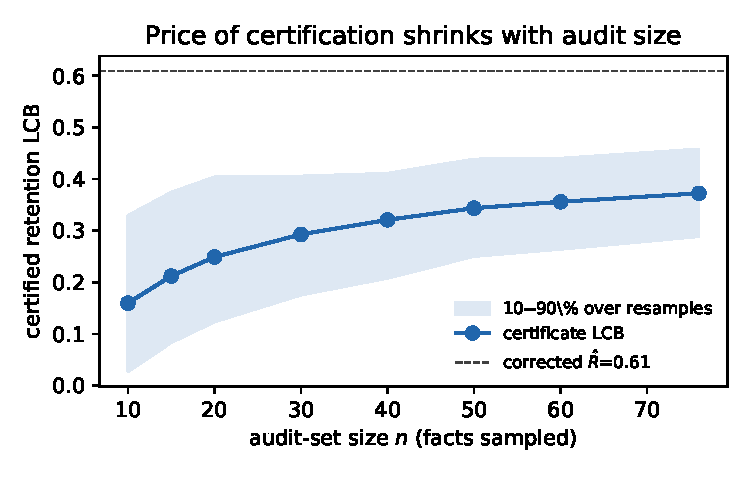
\includegraphics[width=0.31\linewidth]{figures/certify_sizing.pdf}
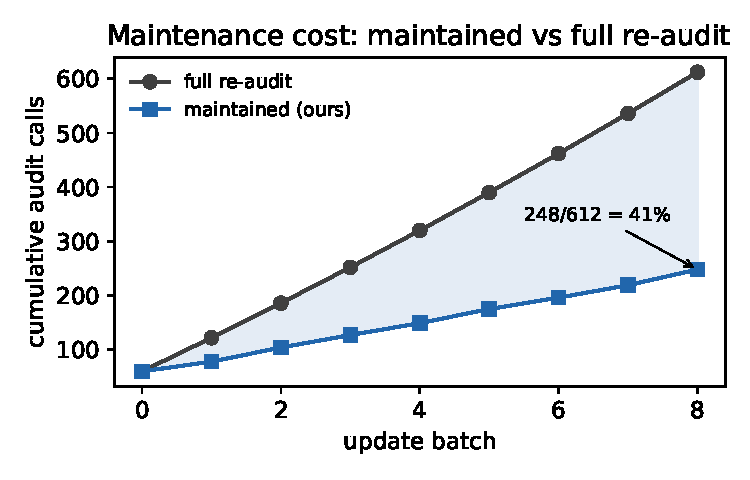
\includegraphics[width=0.31\linewidth]{figures/certify_cost.pdf}
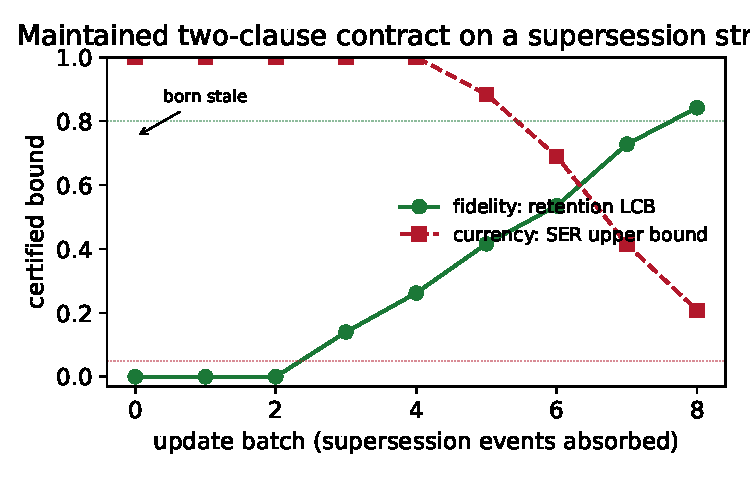
\includegraphics[width=0.31\linewidth]{figures/certify_currency.pdf}
\caption{Left: price of certification (raw estimate minus certified lower bound) vs.\ audit size $n$. Middle: maintained certificate cost vs.\ cumulative full-audit cost across churn batches. Right: maintained fidelity/currency bounds tracking a store from born-stale to current (\S\ref{sec:certify-currency}).}
\label{fig:certify-sizing}
\end{figure}

\subsection{The build lottery: certification matters because point estimates are not reproducible}
\label{sec:build-lottery}

Two independently compiled stores from the \emph{same} corpus, same compiler, same prompt, disagree with each other on $17.1$--$23.3\%$ of per-claim outcomes (measured across two corpus scales, $200$-doc/$25$-page and $400$-doc/$50$-page). One example pair: build A certifies $R \ge 0.327$ while build B's true (oracle) retention is $0.506$ --- either build alone, reported as a point estimate, would mislead in a different direction. This is the concrete justification for certifying with a confidence bound rather than reporting whichever single compile happened to run: LLM compilation is stochastic enough that ``the'' retention of a store is not well-defined without a distribution over builds.

\subsection{Maintaining the certificate as the store changes}

A certificate computed once goes stale as new documents arrive, exactly like the store it describes. We test whether the certificate can be kept valid incrementally, without a full re-audit after every update. On a healthy update stream, maintained certification matches full-audit validity at $40.5\%$ of the query cost ($248$ vs.\ $612$ calls). On an adversarial churn stream (documents arriving fast enough to threaten validity), a stale certificate (last-computed bound LCB $= 0.386$) is breached by batch $7$ as true retention falls to $0.378$; the maintained certificate tracks the decline ($0.357 \to 0.183$) and stays valid throughout, at $85\%$ of full-audit cost ($581$ vs.\ $684$ calls). The certificate is only useful if it is re-validated at the cadence the store actually changes --- a one-time audit would have silently gone stale exactly when it mattered most.

\subsection{The adaptivity trap: self-audited repair overclaims}

A natural response to a low certified score is to repair the store and re-certify. If the repair is \emph{targeted} at the same claims used to detect the problem, the resulting certificate is contaminated by the targeting: a repair-set-audited certificate reads $R = 0.760$ while an honest holdout audit of the same repaired store reads $R = 0.244$ --- a $52$-point overclaim from self-audit alone, with no change to the store's actual quality. The honest fix is not to skip repair, but to avoid auditing on the set that motivated the repair: compiling twice and taking the union of two independent compiles raises the \emph{honest} (holdout) bound from $0.244$ to $0.389$, a genuine $+0.14$ gain, at roughly double the compile cost. This distinction --- overclaiming from self-audit vs.\ a real, if smaller, gain from an honest procedure --- recurs in \S\ref{sec:maintain} as the difference between a maintainer that games its own reward signal and one that does not.

\subsection{Currency under a two-clause contract}
\label{sec:certify-currency}

Combining both clauses on HoH: a store compiled with no currency awareness starts \emph{born-stale} ($R{=}0$, $\mathrm{SER} \le 1.0$ uncertified); after maintenance under the two-clause contract, the certified bounds reach $R \ge 0.842$ and $\mathrm{SER} \le 0.208$, at $47\%$ of full-audit cost ($504$ of $1080$ calls). This is the compile-stage result of \S\ref{sec:compile} restated as a certificate rather than a point estimate: not just ``the compiled store is more current,'' but a stated, auditable confidence bound on how current, kept valid as the store keeps changing.

\section{Maintain: trainable repair under a certified budget}
\label{sec:maintain}

Certification (\S\ref{sec:certify}) tells us \emph{whether} a store is still valid; it does not by itself make maintenance better. This section asks two questions: can the maintainer that rewrites pages under new documents be improved beyond prompting, and can we bound the damage a maintainer causes \emph{as it happens}, rather than only measuring it after the fact.

\subsection{A trained maintainer beats the best prompt, honestly scored}

We compare a minimal offline best-of-$k$ SFT-trained maintainer against the strongest prompted maintainer (\texttt{anchored}) and a vanilla baseline, all at equal deploy cost (single forward pass per rewrite; the SFT cost is paid once, offline). On a $12$-round rewrite protocol ($5$ seeds each), the trained maintainer reaches $R_{12} = 0.523 \pm 0.037$ vs.\ the anchored prompt's $0.397 \pm 0.059$ --- a gain of $+0.127$ (bootstrap $95\%$ CI $[0.067, 0.187]$, Welch $p{=}0.009$) --- against a vanilla baseline of $0.278 \pm 0.052$ and a fresh-rebuild ceiling of $0.552 \pm 0.036$ ($n{=}19$). The trained maintainer recovers $90\%$ of the maintained-vs-rebuild gap, vs.\ $43\%$ (anchored) and $47\%$ (a second, conservative prompt).

We deliberately do \emph{not} claim this result is Pareto-optimal across retention and incorporation (the rate at which new information is successfully written in): the incorporation gain of the trained maintainer over anchored ($0.088$ vs.\ $0.083$) is statistically null (Welch $p{=}0.54$). The honest claim is narrower and still useful: the trained maintainer dominates on retention at incorporation no lower than the prompt's --- not a two-dimensional Pareto win.

\paragraph{A budget-gated boundary for reward gaming.} Offline best-of-$k$ selection could in principle be gamed --- optimizing for whatever proxy signal selects the training data, rather than true fidelity. We measure this directly: the gap between the selection \emph{signal}'s and the resulting \emph{policy}'s gameability rises with how binding the page-length budget is. At a slack budget ($350$ words), the signal-level gameable gap is $0.048$--$0.062$ and the distilled policy's difference-in-differences stays $\approx 0$ ($-0.010$ to $+0.009$); at a binding budget ($120$ words), the signal gap rises to $0.127$--$0.136$ ($\sim\!2.5\times$) while the policy DiD rises only to $0.020$--$0.024$ --- offline distillation ``launders'' roughly $6\times$ of the gameable signal out. We flag two honest weaknesses in this result: the binding-budget policy DiD ($+0.022$) sits below its own estimated binomial noise floor ($\sim 0.038$), so the quantitative $6\times$ figure is a ratio of two small, noisy quantities that could plausibly range from $3\times$ to unbounded; and the \emph{dangerous} half of this boundary law --- what happens under an RL-trained maintainer or a fixed, predictable audit schedule, where gaming the signal is directly the training objective rather than a side effect of selection --- has not been run. We name this as the single largest open risk in the maintenance stage, not as a solved case.

\subsection{LossGate: a per-batch, anytime-valid retention bound}

The trained maintainer above still loses information; \S\ref{sec:certify}'s certificate tells us afterward how much. LossGate instead wraps \emph{any} maintainer (prompted, trained, or otherwise) with a gate-and-rollback wrapper that emits, every batch $t$, a certified worst-case bound $R(t) \ge R(t-1) - b_t$ at confidence $1-\delta$, where $b_t$ is a judge-noise-corrected Clopper-Pearson upper bound on the fraction of previously-confirmed facts destroyed that batch, estimated on a held-out probe pool the maintainer never sees. Per-batch bounds are composed across the full stream via Basel-weighted significance levels ($\alpha_t = \delta \cdot 6/(\pi^2 t^2)$, $\sum_t \alpha_t \le \delta$) into a single \emph{anytime-valid} stream bound $R(t) \ge L_0 - \sum_{s \le t} b_t[s]$ that holds simultaneously at every $t$ with no fixed horizon --- a confidence-sequence guarantee, not a bound computed for one chosen stopping time.

\begin{table}[h]
\centering
\small
\caption{LossGate, 7-seed final numbers. $R(12)$ is retention after 12 batches; paired gain is the per-seed difference between the gated and ungated version of the same maintainer.}
\label{tab:lossgate}
\begin{tabular}{lcc}
\toprule
Maintainer & $R(12)$, ungated & $R(12)$, LossGate-wrapped \\
\midrule
Vanilla prompt & $0.285 \pm 0.05$ & $0.405 \pm 0.09$ (+0.12, $3.4\sigma$, 6/7 seeds positive) \\
Conservative prompt & $0.265 \pm 0.10$ & $0.415 \pm 0.10$ (+0.14, $\sim\!2.7\sigma$, 5/7 seeds positive) \\
\bottomrule
\end{tabular}
\end{table}

Coverage --- the fraction of batches where the certified bound actually held --- is $1.00$ over $168$ gated (arm, seed, batch) cases against a $\ge 0.95$ nominal target, and $0.98$ on an independent judge-free HoH replication. Gating costs $47\%$ additional re-extraction overhead. On a large judge-free probe pool ($n{=}120$), the composed stream lower bound stays strictly positive across all $12$ batches (final LCB $0.07$--$0.13$ against a realized retention of $0.86$); on a smaller pool ($n{\approx}15$), the same bound is valid but loose, hitting zero within roughly two batches even though realized retention stays well above zero. We are explicit that \emph{validity} (the bound never overclaims) and \emph{tightness} (how close the bound is to the truth) are separate properties: LossGate's contribution is the mechanism and the coverage guarantee, not a claim that the bound is tight at every probe-set size.

\begin{figure}[t]
\centering
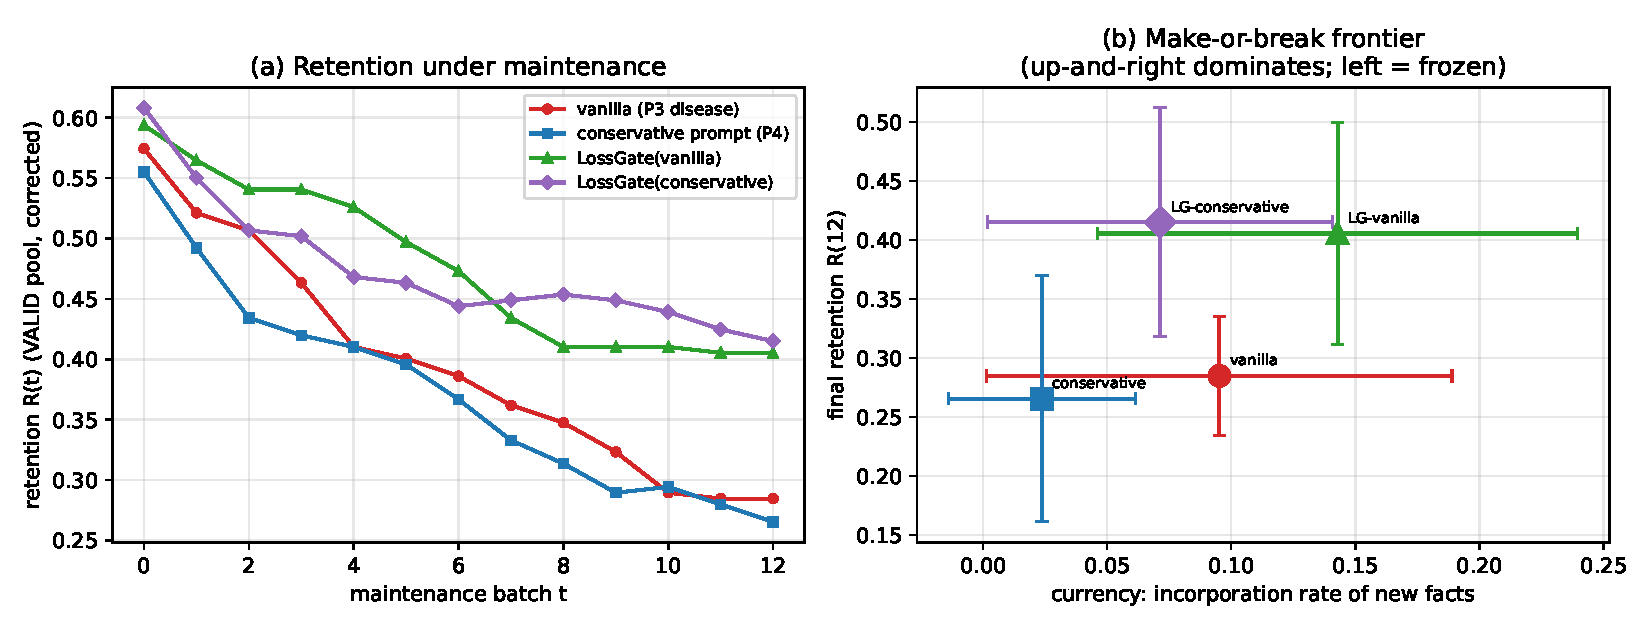
\includegraphics[width=0.48\linewidth]{figures/maintain_frontier.pdf}
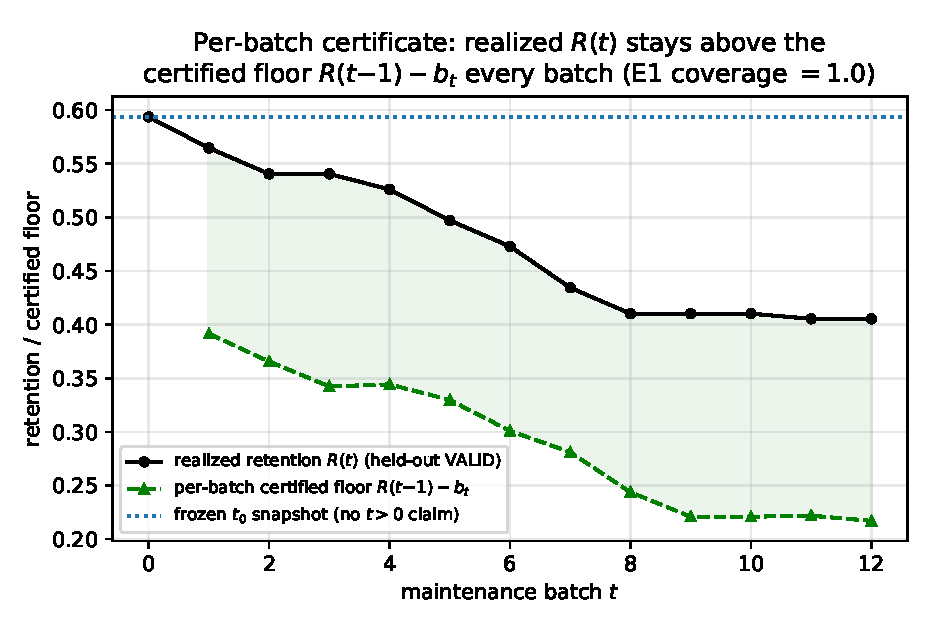
\includegraphics[width=0.48\linewidth]{figures/maintain_stream.pdf}
\caption{Left: retention vs.\ currency frontier across maintainers, gated and ungated. Right: per-batch certified floor $R(t-1) - b_t$ vs.\ realized retention $R(t)$ across the stream.}
\label{fig:lossgate}
\end{figure}

We disclose two scope limitations directly: a second model-scale run was dropped to avoid contending for shared GPUs with other running jobs, not run to completion and discarded, and it is reported as a limitation rather than silently omitted; and the LoRA-wrapped arm (gating around the trained maintainer of \S4.1 rather than a prompted one, retention lifted from $0.405$ ungated to $0.574$ gated) and the rollback-threshold ($\tau$) sweep are each single-seed and noisy, reported as directional rather than confirmed.

\section{Retract: backflow and the membership gate}
\label{sec:retract}

The first three stages assume the store should keep what it has and get better at keeping it. Sometimes a fact must instead be made to leave --- a source is retracted, a user exercises a deletion right, a fact is confirmed wrong. This section asks whether ``deleting'' a fact from a compiled or agentic store actually makes it gone.

\subsection{Backflow: correctness-gated deletion does not stay deleted}

Consider an agent whose memory is not a flat store but a system that periodically \emph{consolidates}: it re-reads its own transcripts and evidence and re-derives and re-writes memory notes, the same rewrite-to-update pattern as \S\ref{sec:compile}--\S\ref{sec:maintain}. If a synthesized private fact $d$ is retracted --- its note deleted --- but the underlying observations that originally supported it are not also purged, we ask whether $d$ resurfaces on a later consolidation pass. We call this \textbf{backflow}.

We test two gate designs at the write-consolidate hook. A \textbf{correctness gate} (A2) admits any write that is faithful to the agent's surviving evidence, regardless of whether that write discloses the retracted fact --- this is the gate design an agent framework would use by default, since it is exactly what ``don't hallucinate, stay faithful to your memory'' asks for. A \textbf{membership veto} (A3) instead blocks any write matching a deletion-set membership predicate (canonicalized-value hash match, or embedding-cone similarity, or NLI entailment of the retracted fact), independent of whether the write is otherwise correct.

On $n{=}250$ synthetic private facts (per-arm $n{=}189$--$221$ after infrastructure-error filtering), the correctness gate leaves residual surfacing at $0.990$ --- statistically indistinguishable from no deletion at all (the no-gate baseline is $0.991$). The membership veto reaches $0.000$ ($95\%$ CI $[0, 0.019]$), matching a never-ingested oracle control. On the subset scored under both gates ($n{=}193$), the discrimination between them is $0.990$ (cluster-bootstrap $95\%$ CI $[0.974, 1.0]$, excluding zero), and two one-sided equivalence tests confirm the gated arm is statistically equivalent to the oracle ($\Delta{=}0.05$, $n{=}189$ pairs). A membership-inference-style audit against the oracle store gives AUC $0.99$ for the leaked (correctness-gated) store and $0.49$--$0.50$ (chance) for the membership-gated store.

\begin{figure}[t]
\centering
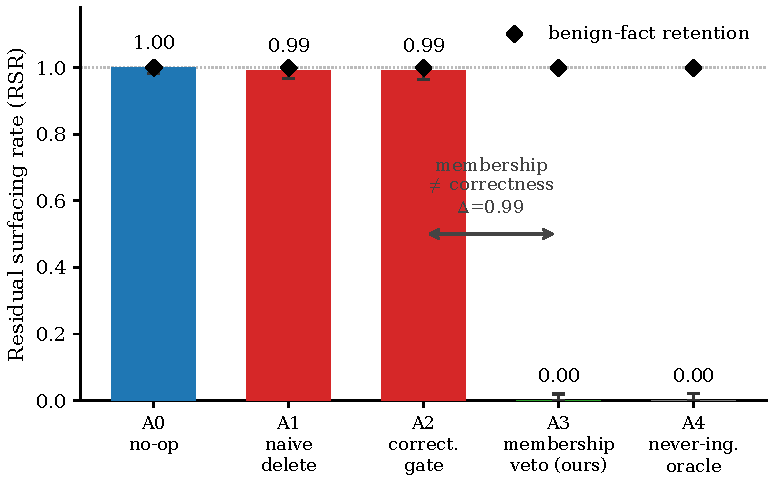
\includegraphics[width=0.48\linewidth]{figures/retract_ladder.pdf}
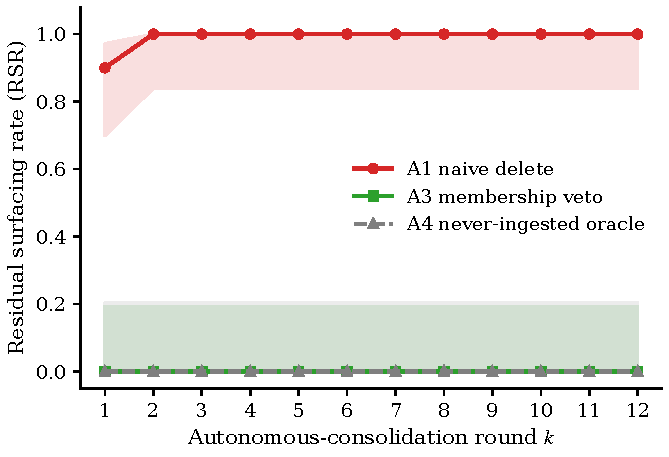
\includegraphics[width=0.48\linewidth]{figures/retract_ksweep.pdf}
\caption{Left: residual surfacing rate across the A0 (no-op)--A4 (never-ingested oracle) arm ladder. Right: surfacing rate across 12 rounds of native consolidation --- the correctness-gated arm rises back toward the no-deletion baseline within two rounds; the membership-gated arm stays flat at zero.}
\label{fig:retract-ladder}
\end{figure}

\paragraph{Scope.} We replicate the effect under the agent's own native (auto-triggered) consolidation loop, not only a scripted harness, and probe a second, architecturally distinct memory substrate (a block-plus-archival agent architecture). We state the scope of that second-substrate result precisely rather than as a second full replication: it is a directional probe ($n{=}24$) with a noisy no-op control ($A0{=}0.88$ rather than the expected $\approx\!1.0$), and it tests the architecture's memory blocks rather than its full agentic tool-call loop. We describe the overall evidence as \emph{two substrates plus a directional second-model probe}, not two independent paradigms or two model families confirming each other --- the $n{=}24$ evidence supports this narrower framing and no stronger one.

\subsection{A complementary result: refusing leakage at serving time}

We additionally target a related but distinct problem: even with a sound deletion gate at the write path, a backbone model may still leak a retracted fact from its own parametric memory when asked directly, independent of what the compiled store contains. We build a serving-time refusal gate for compiled wikis and measure it against a RAG-drop baseline (removing the source's chunk from the retrieval index, but not gating the model's own recall): on correct-and-retracted queries, the gated system leaks $0\%$ of the time against $100\%$ for the RAG-drop baseline. This is an architectural result --- the gate refuses by construction, the RAG-drop baseline surfaces by construction --- and is independent of any statistical estimator. We report it with its own honest caveats: the correct-and-retracted stratum is small ($n{=}15$), giving a wide confidence interval, and the backbone and the judge share the same underlying model family, a circularity risk we flag explicitly.

We also explored a formal criterion for a harder case: a claim in the compiled wiki whose content is \emph{fused} from two or more sources, so that retracting one source cannot be done by deleting a single sentence. We do not carry that formal criterion into this paper. Our own analysis found the proposed residue metric structurally blind to exactly the fused-claim case it was built to detect: by the metric's own definition, a fused claim already has no single source that entails it above threshold, which is also the condition the residue check uses to declare success --- so the metric cannot distinguish a claim that correctly dropped the retracted source's contribution from one that never could have revealed it. We do not use it. \textbf{Formally certifying removal of one source's marginal contribution to a claim that several sources jointly support remains an open problem}, and we name it as such rather than presenting a partial or contested solution as settled.

\section{Discussion}
\label{sec:discussion}

\begin{table}[h]
\centering
\small
\caption{The lifecycle: one mechanism and one headline number per stage, with the limitation that most bounds its generality.}
\label{tab:lifecycle}
\begin{tabular}{p{1.7cm}p{3.6cm}p{3.9cm}p{4.3cm}}
\toprule
Stage & Mechanism & Headline number & Key limitation \\
\midrule
Compile & recency-aware supersession resolution & SER $0.007$ vs.\ $0.177$--$0.280$ baselines ($n{=}300$) & single build, no seed variance \\
Certify & noisy-judge-corrected $(\delta,\varepsilon)$ confidence bound, incrementally maintained & maintained validity at $40$--$47\%$ of full-audit cost & compiler family varied only on the fidelity gate \\
Maintain & offline-trained maintainer + per-batch anytime-valid rollback gate & $+0.127$ retention over best prompt ($p{=}0.009$); LossGate $+0.12$--$0.14$ & dangerous half of the reward-gaming boundary law untested; 2nd model scale dropped \\
Retract & membership-keyed write veto vs.\ correctness-keyed gate & $0.990 \to 0.000$ residual surfacing & second substrate is an $n{=}24$ directional probe; fused-claim retraction is open \\
\bottomrule
\end{tabular}
\end{table}

Three patterns recur across stages independently of the specific benchmark or model. First, \emph{resolution beats accumulation}: a system that overwrites/resolves rather than appends is what fixes staleness (\S\ref{sec:compile}), and the same overwrite-vs-append distinction is what makes membership-gated retraction durable against a correctness-gated one that merely appends a veto (\S\ref{sec:retract}). Second, \emph{self-audit is not audit}: the adaptivity trap (\S\ref{sec:certify}) and the reward-gaming boundary in trained maintenance (\S\ref{sec:maintain}) are the same failure at two different stages --- a system that grades its own repair, or trains on its own selection signal, will look better than it is unless the audit set is held genuinely independent. Third, \emph{a bound that is valid but loose is still useful}: both the currency certificate (\S\ref{sec:certify}) and LossGate (\S\ref{sec:maintain}) are explicitly not tight at small sample sizes, and we treat that as a disclosed scope limitation rather than a reason to drop the confidence-bound framing --- a loose-but-valid bound is still strictly more informative than a point estimate with no bound at all.

What does not yet generalize: every stage's primary evidence comes from a small number of model families (mostly Qwen2.5/3), one or two benchmarks, and in most cases a single build or seed count too small to report full seed-variance statistics. We view the lifecycle framing itself --- compile with resolution, certify with a maintained confidence bound, maintain with a certified rollback gate, retract with a membership-keyed veto --- as the contribution most likely to generalize beyond these specific numbers, since the same overwrite-vs-accumulate and self-audit-vs-independent-audit distinctions appear at every stage we tested it at.

\section{Limitations}
\label{sec:limitations}

We list every limitation identified during the writing of this paper, organized by stage, rather than folding them into a single generic paragraph. This paper has not been externally peer-reviewed; the items below are what our own scrutiny of each result surfaced.

\textbf{Compile (\S\ref{sec:compile}).} The HoH result is a single build and a single run: no seed variance is reported for the compile step itself, so we cannot separate genuine effect size from build-to-build noise at the level \S\ref{sec:build-lottery} shows exists for the compiler in general. The scaled substrate is HoH-only; a second substrate (source code libraries) is a small consistent check ($n{=}14/13$), not a powered second benchmark. A static-audit cross-pipeline probe using a different reader, embedder, and substrate (SciFact-Open) is directional, not a controlled comparison, because the intended matched-pipeline version could not be run (a shared-GPU thread-limit conflict with other jobs on the host). The external-validation experiment (\S\ref{sec:compile-external}) is single-seed and self-judged by the same model that performed the rewrite, at temperature $0$; an independent, calibrated judge pass for that specific experiment has not been run.

\textbf{Certify (\S\ref{sec:certify}).} The compiler/judge model family is varied (Qwen vs.\ Llama) only for the fidelity gate experiment; every other certified number in this section uses Qwen for both compiler and judge, so cross-family generality of the maintained-certificate and adaptivity-trap results specifically is untested. Judge-noise calibration uses a constructed present/absent pair set, not human-labeled data. The dense-RAG comparator uses oracle page routing, isolating page-content fidelity from retrieval-routing error --- a real deployed RAG system would also incur routing loss that this comparison does not charge it for.

\textbf{Maintain (\S\ref{sec:maintain}).} The single largest open risk in this paper: the boundary law's dangerous regime (an RL-trained maintainer, or a maintainer facing a fixed and predictable audit schedule, where gaming the audit signal is the direct training objective rather than a side effect of offline selection) has not been run, only predicted by extrapolation from the offline-selection regime. The binding-budget policy difference-in-differences ($+0.022$) is below its own estimated noise floor, so the $\sim\!6\times$ signal-laundering ratio should be read as directional, not precise. A second model scale was not run, for a disclosed reason (avoiding GPU contention with others' concurrent jobs), not because it was attempted and failed. The LoRA-wrapped LossGate arm and the rollback-threshold sweep are each single-seed.

\textbf{Retract (\S\ref{sec:retract}).} The primary $n{=}250$ ladder result uses one composition template and one primary model (Qwen3-14B); the second-model probe (Llama) is $n{=}24$ with a noisy no-op control and tests a different memory architecture's block-plus-archival substrate rather than a matched second run of the same experiment. We do not consider ``two substrates plus a directional probe'' equivalent to ``validated across two model families,'' and say so explicitly rather than letting the stronger-sounding framing stand. The complementary serving-time leakage-refusal result has a small correct-and-retracted stratum ($n{=}15$) and shares a model family between backbone and judge. Formally certifying retraction of a claim whose content is fused across multiple sources is, as stated in \S\ref{sec:retract}, an open problem this paper does not solve --- we considered a formal residue-metric criterion for this case and found it structurally unsound (\S\ref{sec:retract}), so we do not carry it forward as a claim, rather than present a contested result as settled.

\textbf{Cross-cutting.} Every stage's headline experiments were run under a shared-GPU, non-disruptive-use policy that occasionally forced a scale-up or a second run to be skipped rather than delayed indefinitely; we have tried to flag every instance where this affected a specific result rather than only mentioning the policy once here. No stage in this paper has had a genuinely external (non-author) peer review pass; the checks we ran ourselves are what shaped which results are reported and how.

\section{Related work}
\label{sec:related}

\paragraph{Compiled knowledge stores.} The LLM-Wiki pattern we study originates with \citet{karpathy2026wiki}. Closest prior work on certifying compiled stores is \citet{wicer} (iterative wiki-memory compile-evaluate-refine) and \citet{streaming} (proactive materiality-scored pinning for time-evolving compiled stores), neither of which ships a statistical certificate of the kind in \S\ref{sec:certify}; \citet{cochran2026wikirag} independently benchmark vector RAG against an LLM-compiled wiki on a smaller multi-domain corpus, consistent in direction with \S\ref{sec:compile} but without the structure-vs-resolution dissociation. Graph- and tree-structured RAG systems --- LightRAG \citep{guo2025lightrag} and RAPTOR \citep{sarthi2024raptor} --- are the real accumulating-structured baselines we compare against directly rather than re-implement.

\paragraph{Conformal and finite-sample certification.} Our $(\delta,\varepsilon)$ contract follows the general conformal-prediction and PAC-style finite-sample certification tradition, most directly \citet{conformal}'s conformal importance guarantees for summarization; \citet{schuirmann1987tost}'s two one-sided tests procedure underlies the equivalence claim in \S\ref{sec:retract}. Sequential and anytime-valid inference --- the confidence-sequence structure LossGate's stream bound uses --- follows the betting/e-process line of work on bounded-random-variable estimation.

\paragraph{Model editing and knowledge maintenance.} Localized parameter editing \citep{meng2022rome,meng2023memit} and surveys thereof \citep{yao2023editing} address a related but distinct problem: updating a model's weights rather than a compiled text store. \citet{gupta2024editing} document catastrophic forgetting under repeated large-scale edits, a weight-space analogue of the rewrite-damage phenomenon we measure in text stores (\S\ref{sec:compile}, \S\ref{sec:maintain}); \citet{lyaplock2025} study bounded knowledge preservation in sequential editing with a Lyapunov-style stability argument, complementary to our empirical per-batch bound. Retrieval-side dynamic-corpus benchmarks include \citet{liska2022streamingqa} and the HoH benchmark \citep{ouyang2025hoh} we build on directly.

\paragraph{Model and retrieval collapse.} \citet{shumailov2024collapse} and \citet{gerstgrasser2024collapse} study collapse under recursive training on model-generated data; \citet{modelcollapse2025} and \citet{retrievalcollapse} extend this to knowledge fidelity and retrieval quality specifically under recursive synthetic pollution. Our compile- and maintenance-stage decay results are a related but distinct phenomenon --- information loss under repeated \emph{editorial rewriting} of a fixed underlying fact set, not training-distribution collapse from synthetic data --- but the failure mode (fluent output, silently wrong or missing content) rhymes closely enough that we treat this as the closest adjacent literature.

\paragraph{Machine unlearning and retraction.} Benchmark-style unlearning work \citep{maini2024tofu,shi2024muse,jin2024rwku,chen2024flat} and the broader unlearning survey \citep{bourtoule2021machine} target weight-level forgetting, evaluated by whether a model's output distribution changes; \citet{eldan2023whosharrypotter} and \citet{ye2024harrypotterleak} probe residual leakage after unlearning specifically. \citet{pawelczyk2024incontext} study in-context (prompt-level, not weight-level) unlearning. \citet{agenticunlearning2026} is the closest prior work to \S\ref{sec:retract}'s setting --- unlearning inside an LLM-agent memory loop rather than a static model --- though it does not identify or measure the backflow phenomenon via autonomous consolidation that is this section's central finding. \citet{liu2024unlearnrag} study unlearning for RAG systems specifically, a serving-time-retrieval analogue of the write-time retraction problem we study. Deletion under database-style privacy guarantees \citep{inference2026deletion} and cognitive-memory-architecture forgetting benchmarks \citep{forgetful2026} are adjacent settings without the agent-consolidation mechanism central to backflow.

\paragraph{Agent memory systems.} Mem0 \citep{chhikara2025mem0} and MemGPT/Letta \citep{packer2023memgpt} are the two agent-memory architectures we test the membership-veto mechanism against as the primary and secondary substrates in \S\ref{sec:retract}, unmodified except for the write-hook gate we add.

\section{Conclusion}
\label{sec:conclusion}

A compiled knowledge store is not safer than RAG by default; it is only as safe as the four things it does with what it compiles. We found that resolving supersession, not adding structure or memory, is what actually fixes staleness at compile time; that a statistical contract is needed because compiled stores are stochastic enough that two identical-looking builds can disagree on a fifth of their claims; that maintenance can be made partially trainable and wrapped in a certified rollback gate, but that the gate's value is in bounding damage as it happens rather than only measuring it afterward; and that deleting a fact from an agentic memory does not make it stay deleted unless the deletion gate is keyed on what the fact \emph{is} rather than on whether a later write happens to be correct. Several of the numbers in this paper come from single seeds, single model families, or single builds, and we have tried throughout to say so plainly rather than let a strong-sounding headline stand unqualified. We release the code for every stage, and consider the clearest next step to be closing the gaps this paper names explicitly: seed variance in compilation, the untested dangerous half of the maintenance boundary law, and a formal treatment of retracting claims fused across multiple sources.


\bibliography{references}
\bibliographystyle{iclr2026_conference}

\end{document}
